\chapter{Text Mining}\label{Text Mining}

Nu we een algemeen begrip hebben van wat machine learning juist is en welke algemene technieken het omvat, kunnen we overgaan naar text mining en zijn geschikte technieken. Dit hoofdstuk bespreekt welke technieken we kunnen gebruiken voor text mining en wat deze juist inhouden. Als laatste gaan we de theorie toepassen op een proefopstelling en gaan we de resultaten van dit experiment bespreken. 
\newline
%
Text mining of text data mining is een techniek waarbij men aan tekstanalyse doet om zo trends en patronen te kunnen vaststellen. Neem opnieuw als voorbeeld onze artikels. Met text mining wil men de artikels zodanig analyseren dat men kan uitmaken welke artikels positief en welk negatief zijn.
Een probleem dat zich onmiddelijk bij text mining voordoet is het ontbreken van een  \'e\'en-op-\'e\'en relatie van woorden en een concept. Woorden verwijzen zelden eenduidig naar \'e\'en concept. Zo kan het voorkomen van het woord "bank" in een tekst zowel verwijzen naar de financi\"ele instelling als naar een doodgewone zitbank in het park. Dergelijke dubbele betekenis van woorden maakt het moeilijk om de woorden, met als gevolg ook de tekst, te mappen op een bepaald concept.
% 
Verder heeft men ook woorden in een tekst die weinig bijdragen tot de bepaling van het concept van de tekst bijvoorbeeld: ik,en,want...
Deze woorden kan men uit de tekst filteren door een database aan te leggen met woorden die men moet negeren. Deze techniek en nog soortgelijke alternatieven vereisen dat er al een voorverwerking plaatsvindt voordat men de dataset echt gaat analyseren op patronen en trends. Dit noemt men \textbf{\textit{document pre-processing}}.

\section{Document Pre-processing }\label{Document Pre-processing}

Document pre-processing is een optionele, maar zeker nuttig stap in het text mining proces. Document pre-processing bestaat eruit om de dataset al eens gaat verwerken voor het te laten analyseren door het algoritme, zodanig dat men extra informatie heeft  die men kan gebruiken bij de eigelijke analyse van de dataset. Zo kan men bijvoorbeeld alle stopwoorden verwijderen uit de dataset. Wanneer men dan op deze gewijzigde dataset een analyse uitvoert, geeft men indirect de informatie mee dat stopwoorden er niet toe doen. Uiteraard is het verwijderen van stopwoorden \'e\'en van de technieken.  Er bestaan nog andere technieken die nuttig zijn als voorverwerking van een dataset. Zo kan men tekst en structuren afleiden. Bijvoorbeeld het omzetten van Microsoft Word of Latex documenten naar XML maakt het parsen en analyseren van de documenten voor het algoritme veel gemakkelijker.Verder kan men ook \textbf{\textit{stemming}} toepassen. Stemming is een techniek waarbij men tracht om de stam van het woord te achterhalen. Bijvoorbeeld uit het woord \textit{katachtig} kan men het woord \textit{kat} afleiden. De techniek kan gebaseerd zijn op een woordenboek bijvoorbeeld \textit{Mmorph} \cite{petitpierre1995mmorph} is zo'n stemmingswoordenboek. Verder kan men de stemming ook baseren op een set van regels, bepaald door taalkundige. Het onderstaande voorbeeld illustreert een set van stemming regels voor het Frans:
%Voorbeeld van stemming regels   
\begin{center}
  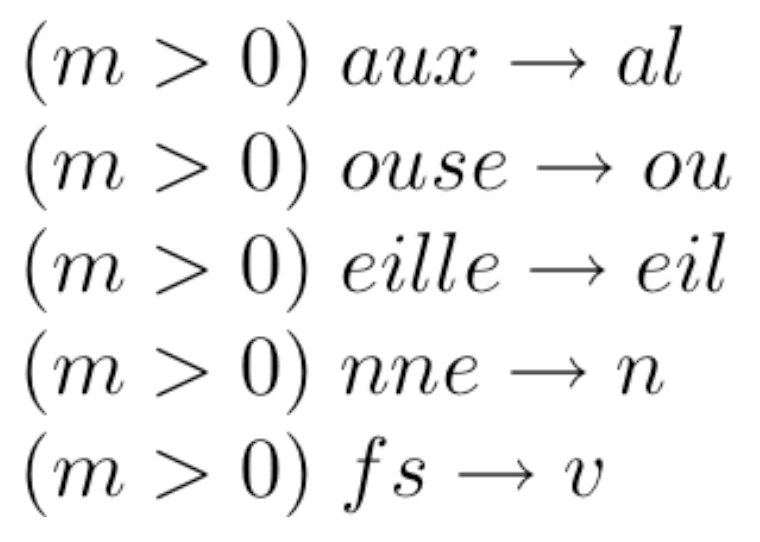
\includegraphics[width=5cm]{stemming_regels_frans}
  \captionof{figure}{Voorbeeld van stemming regels in het Frans}
\end{center}
%%
Tenslotte is \textbf{\textit{named entity recognition}} (NER) ook een techniek die men gebruikt bij document pre-processing. Hierbij gaat men entiteiten proberen te detecteren in de tekst en deze labelen. Neem bijvoorbeeld de zin \textit{Yannick heeft zich ingeschreven in de richting Computerwetenschappen aan de Vrije Universiteit Brussel in 2012}. Men kan met NER de entiteiten eruit halen, labelen en volgend resultaat verkrijgen:\\ \textit{$\text{[Yannick]}_{persoon}$ heeft zich ingeschreven in de richting Computerwetenschappen aan de $\text{[Vrije Universiteit Brussel]}_{organisatie}$ in $\text{[2012]}_{tijdsaanduiding}$}
\newline
Algemeen kan men stellen dat een combinatie van deze technieken alleen maar de uiteindelijke resultaten ten goede komt. Hoe deze gecombineerd kunnen worden, wordt in het onderstaande voorbeeld ge\"illustreerd. 
\begin{center}
  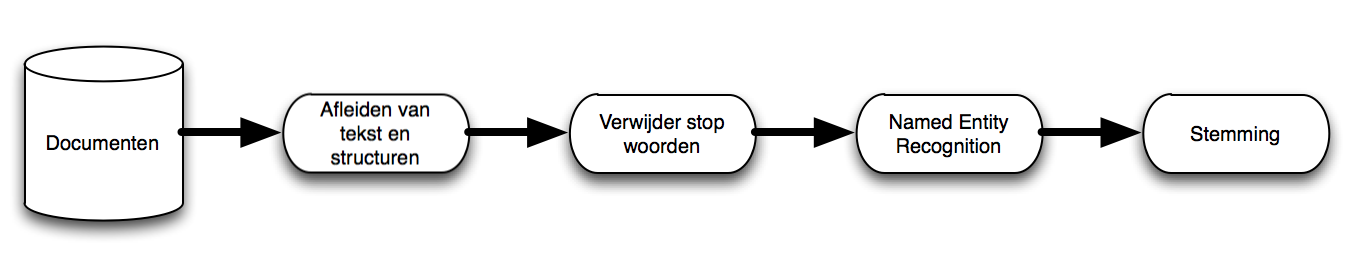
\includegraphics[width=10cm]{document_preprocessing}
  \captionof{figure}{Combinatie van technieken bij document pre-processing}
\end{center}
%
\section{Methoden}\label{Methoden}
Na de document pre-proccesing kunnen we beginnen aan de eigelijke analyse van de dataset. Voor de text mining kunnen we de vector space methode gebruiken.
\subsection{Vector Space Methode}\label{Vector Space Methode}
De vector space methode is een methode waarbij we een document als een vector voorstellen waarbij ieder element overeenkomt met een woord en zijn frequentie in het document. De elementen van de vector worden ook wel features genoemd. Als men concreet een document voorstelt kan men zeggen dat document $j$ voorgesteld wordt door $\textbf{d}_{j}$ met $f_{ij}$ de frequentie van het woord $w_{i}$. Met de frequentie $f_{ij}$ bedoelt men het totaal aantal voorkomens van het woord $w_{i}$ in document $j$. Het aantal verschillende woorden in het document stelt men voor door $n_{w}$, wat eveneens de dimensie is van de vector.
Het document $j$ kan dus als volgt worden voorgesteld:
%
\[ d_{j}  = \begin{bmatrix}
    f_{1j} \\
    f_{2j} \\
    \vdots \\
    f_{n_{w}j} \\
\end{bmatrix}  
\]
%
Een belangrijk inzicht bij het vector space methode is dat een document voorgesteld wordt als een groep van woorden. Er wordt geen rekening gehouden met de volgorde waarin de woorden in het document voorkomen. Vaak ziet men ook dat de vector vaak ijl is en vanwege de grote hoeveelheid aan woorden in een document heel groot. Als we nu niet \'e\'en document maar meerdere documenten nemen en we zeggen dat het aantal documenten gelijk is aan $n_{d}$. Dit resulteert in een matrix waarbij iedere kolom een document voorstelt.
\[
D =
 \stackrel{\mbox{Documenten}}{%
    \begin{bmatrix}
    f_{11} & f_{12} & \cdots & f_{1n_{d}} \\
    f_{21} & f_{22} & \cdots & f_{2n_{d}} \\
    \vdots & \vdots & \ddots & \vdots \\
    f_{n_{w}j} & f_{n_{w}2} & \cdots & f_{n_{w}n_{d}}
    \end{bmatrix}
    }
    & Woorden \]
%
Deze matrix wordt een \textbf{\textit{terms-documents matrix (TDM)}} genoemd. Wanneer men spreekt van een  \textbf{\textit{documents-terms matrix (DTM)}}, spreekt men een getransponeerde terms-documents matrix. Een rij van een DTM stelt dan een document voor.
%
De voorstelling brengt ons dichter bij het vinden van een verband tussen documenten.
We kunnen aan de hand van de euclidische afstand bepalen of documenten gelijkaardig zijn of niet. Stel men heeft twee documenten met een kleine euclidische afstand. Dit wil eigelijk zeggen dat de vectorvoorstelling van de documenten gelijkaardig is. Wat wil zeggen dat de woordfrequenties ongeveer overeen komen en dus bijvoorbeeld de documenten over hetzelfde onderwerp gaan of eenzelfde mening uitdrukken.
%
In de praktijk is gebleken dat documenten vergelijken op basis van woordfrequentie niet altijd de gewenste resultaten oplevert. Vaak is het nog altijd moeilijk om verschillend groepen tussen de documenten te onderscheiden. Daarom kan men nog extra verfijningen toepassen aan de hand van \textbf{\textit{term weighting}} en \textbf{\textit{Latent Semantic Models (LSM)}}.


\subsubsection{Term weighting}\label{Term weighting}

Als men even stil staat bij onze TDM met woordfrequenties, kan men zeggen dat niet elk woord evenveel doorweegt. Een woord dat in alle documenten voorkomt biedt geen of minder waardevolle informatie, dan een woord dat zelden voorkomt. En hierop baseert term weighting zich. Het gaat een wegingsfactor introduceren. Ieder woord krijgt een gewicht toegewezen, dat weergeeft hoe belangrijk het woord is. Neem als voorbeeld een hoop recensies van de film "Pulp Fiction" en de woorden "Pulp" en "excellent". "Pulp" is een woord dat voorkomt in de titel van de film en komt ongetwijfeld in elke recensie voor. "Excellent" daarentegen is een woord dat enkel maar voorkomt wanneer de recensist de film fantastisch vond, het zal niet in elk document voorkomen en is waardevolle informatie. Term weighting zal dus bij dit voorbeeld "excellent" een grotere gewicht toewijzen als "Pulp". 
%
De kwantiteit van dit gewicht wordt vaak de \textbf{inverse document frequency  (idf)} genoemd en wordt bepaald aan de hand van volgende formule:
\[w_{i}: idf_{i} = -log_{2}[P(w_{i})] \]
met $P(w_{i})$ de priori probability dat woord $w_{i}$ voorkomt in het document.\\
%
De inverse document frequency geeft het algemeen belang van het woord $w_{i}$ weer. Men kan dit benaderen door het logaritme te nemen van het aantal documenten waar $w_{i}$ in voorkomt en het totaal aantal documenten.
Een andere nuttige kwantiteit is de  \textbf{term frequency} $tf_{ij}$. Deze geeft het belang weer van het woord $w_{i}$ binnen in het document $d_{j}$  en wordt als volgt genoteerd:
\[ tf_{ij} = \frac{f_{ij}}{ \sum_{i=1}^{n_{w}}f_{ij}} \]
%
$tf_{ij}$ wordt berekend door de frequentie, het aantal voorkomens, van een woord $w_{i}$ in document $d_{j}$ te delen door de som van alle woordfrequenties in document $d_{j}$.
Met deze twee kwantiteiten kan men een nieuwe begrip introduceren: de \textbf{tf-idf score}. Wat overeenkomt met het product van tf en idf.
\[ \text{tf-idf score} = tf . idf_{ij} = idf_{i} . tf_{ij} \]
%
De tf-idf matrix bekomt men dan door alle woordfrequenties van het terms-document matrix te vervangen door de tf-idf score.
Deze matrix wordt bijvoorbeeld vaak gebruikt om de gelijkenissen tussen twee documenten te bepalen op basis van cosinusgelijkenis.
%
\subsubsection{Latent Semantic Models}\label{Latent Semantic Models}

Als tweede verfijning van het vector space model, hebben we latent semantic models (LSM). Met LSM probeert men een notie te krijgen van de semantische informatie en meer bepaald het semantisch verband tussen woorden. Bijvoorbeeld als we zoeken naar documenten met het woord "economie", willen we ook documenten met "financi\"en" terugkrijgen. Voor LSM zijn twee woorden semantisch gerelateerd als ze gebruikt worden in dezelfde context. Met het concrete voorbeeld kunnen we zeggen dat er een semantisch verband is tussen 2 woorden als ze vaak voorkomen in dezelfde documenten.
\newline
Merk op dat bij Latent Semantic Models het wederom belangrijk is dat ieder woord naar \'e\'en concept verwijst.
%
\newline
Analytisch wordt LSM toegepast door \textbf{Singular Value Decomposition (SVD)} toe te passen op de terms-document matrix. SVD is een concept uit de lineaire algebra en zegt dat een matrix A opgesplitst kan worden als een product van matrixen namelijk \\
\[A = U\Sigma V^T \]
De reductie van de dimensie gebeurt aan de hand van volgend principe
%
%afbeelding van SVD in latex
\newcommand{\vect}{\mathbf}
\newcommand{\nul}{\operatorname{Nul}}
\newcommand{\col}{\operatorname{Kolommen }}
\newcommand{\row}{\operatorname{Rijen}}
\[
   A= U\Sigma V^T=
  \begin{matrix}
    \underbrace{\left[\begin{matrix}\vect u_1 & \vect u_2 & \dots & \vect u_r\end{matrix}\right.}& 
    \underbrace{\left.\begin{matrix}\vect u_{r+1} & \dots &  \vect u_m\end{matrix}\right]}\\
    \col A & \nul A^T
  \end{matrix}
  \begin{bmatrix}
      \sigma_1 & 0 & \dots & 0 & 0 & \dots & 0 \\
         0 & \sigma_2  & \dots & 0 & 0 & \dots & 0 \\
         \dots& & & & &  \\
         0 & 0 & \dots & \sigma_k  & 0 & \dots & 0 \\
         0 & 0 & \dots & 0 & 0 & \dots & 0 \\
         \dots& & & & &  \\
         0 & 0 & \dots & 0 & 0 & \dots & 0 
  \end{bmatrix}
  \begin{bmatrix}
    \vect v_1^T \\ \vect v_2^T \\ \dots \\ \vect v_r^T \\
    \vect v_{r+1}^T \\ \dots \\ \vect v_n^T
  \end{bmatrix}
  \begin{matrix}
    \left.\vphantom{\begin{bmatrix}
       \vect v_1^T \\ \vect v_2^T \\ \dots \\ \vect v_r^T 
       \end{bmatrix}}\right\}\row A \\ 
    \left.\vphantom{\begin{bmatrix}
      \vect v_{r+1}^T \\ \dots \\ \vect v_n^T 
    \end{bmatrix}}\right\}\nul A
  \end{matrix}
\] 
\newline
U is de unitaire matrix waarbij men $u_1, u_2, ... , u_n$ de linker singuliere vectors noemt. Deze stellen een document met zijn features voor. $V^T$ is de geconjugeerde getransponeerde matrix van V. $v_1, v_2, ... , v_n$ noemt men de rechter singuliere vectors en stellen de woorden met hun features over alle documenten voor. $\Sigma$ is diagonaal matrix met singuliere waarden $\sigma_1,\sigma_2,..,\sigma_n$'  op de diagonaal. De reductie van een term-document matrix naar een dimensie van $K$ gebeurt door de hoogste $K$ singuliere waarden te nemen in $\Sigma$ met de overeenkomstige singuliere vectoren uit $U$ en $V$.    
Doordat men de dimensionaliteit van de vectoren kan beperken door semantisch gelijkaardige woorden bijeen te voegen. Laat dit het toe om een soort van context groepen te cre\"eren en zo een zeker inzicht te krijgen in de dataset. Het is dan ook gebleken dat SVD toepassen een zeer nuttige eerste stap is bij text mining \cite{maas2011learning} omdat men nieuwe meer effici\"ente features krijgt. De nieuwe features geven meer duidelijkheid en inzicht en kunnen dienen als input voor een machine learning algoritme dat probeert text te analyseren bijvoorbeeld bij classificatie of sentiment prediction.
